% ------------------------------------------------------------------------
% file `uaa_radicaux_pythagore_trigonometrie-exercise-9-exercise-body.tex'
%   in folder `xsim/'
%
%     exercise of type `exercise' with id `9'
%
% generated by the `exercise' environment of the
%   `xsim' package v0.20c (2021/02/03)
% from source `uaa_radicaux_pythagore_trigonometrie' on 2021/12/01 on line 171
% ------------------------------------------------------------------------
    Ci-dessous, une pyramide régulière à base carrée. Les côtés du carré mesurent 4cm et les arêtes de la pyramide mesurent 7cm. Détermine la hauteur de cette pyramide.\\
    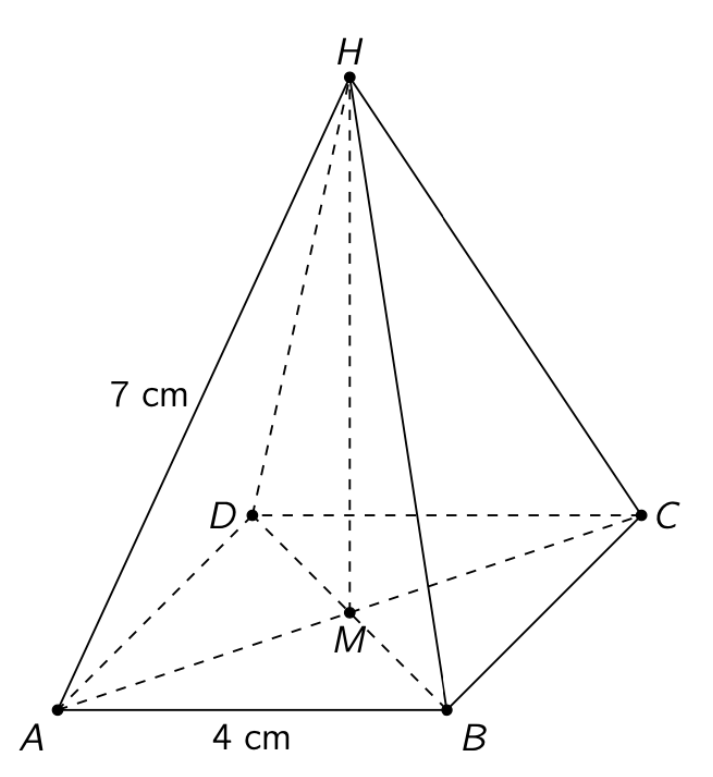
\includegraphics[width=6cm]{img/Q14.png}

